\begin{center}
\textbf{Лабораторная работа №5}
\\
\textbf Работа с пакетным менеджером для С++
\\
\end{center}
\textbf{Порядок выполнения:} 
\begin{enumerate}
\item Запустить VS.
\item Создать проект С++ -> CMake. При создание проекта снять флажок “Создать папку для проекта”.
\item Выполнить сборку созданного проекта
\item Открыть главный CMakeLists.txt (в самой верхней папке)
\item До строки add\_executable добавить
find\_package(CPPAN REQUIRED)
cppan\_add\_package(
	pvt.cppan.demo.intel.opencv.highgui-3
)
cppan\_execute()
\item После строки
 add\_executable добавить
target\_link\_libraries
(ПервыйАргументИзAddExecutable
	pvt.cppan.demo.intel.opencv.highgui
)
\item В файле с кодом (.cpp файл) подключить заголовочный файл
#include <opencv2/highgui.hpp>
\item В функцию main() добавить код для открытия изображения в формате png и сохранения файла в формате bmp.

 
\\
\end{enumerate}
\newpage
CMakeProject1.cpp:\\
// CMakeProject1.cpp: определяет точку входа для приложения.\\
//
\#include <opencv2/highgui.hpp>\\
\#include "CMakeProject1.h"\\

using namespace std;\\

int main()\\
{
	cout << "Hello CMake." << endl\\
	auto i = cv::imread("E:\\student\\picta.png");\\
	i = 255 - i; // инверсия изображения\\
	cv::imwrite("E:\\student\\img.bmp", i);
\\
	return 0;\\
}



\newpage
CMakeList.txt:\\

\# CMakeList.txt: проект CMake для CMakeProject1; включите исходный код и определения
\# укажите здесь логику для конкретного проекта.
\#
cmake\_minimum\_required (VERSION 3.8)

find\_package(CPPAN REQUIRED)
cppan\_add\_package(
	pvt.cppan.demo.intel.opencv.highgui-3
)
cppan\_execute()

\# Добавьте источник для исполняемого файла этого проекта.
add\_executable (CMakeProject1 "CMakeProject1.cpp" "CMakeProject1.h")

\# TODO: Добавьте тесты и целевые объекты, если это необходимо.
			
target\_link\_libraries(CMakeProject1 pvt.cppan.demo.intel.opencv.highgui)


\begin{figure}[h]
\centering
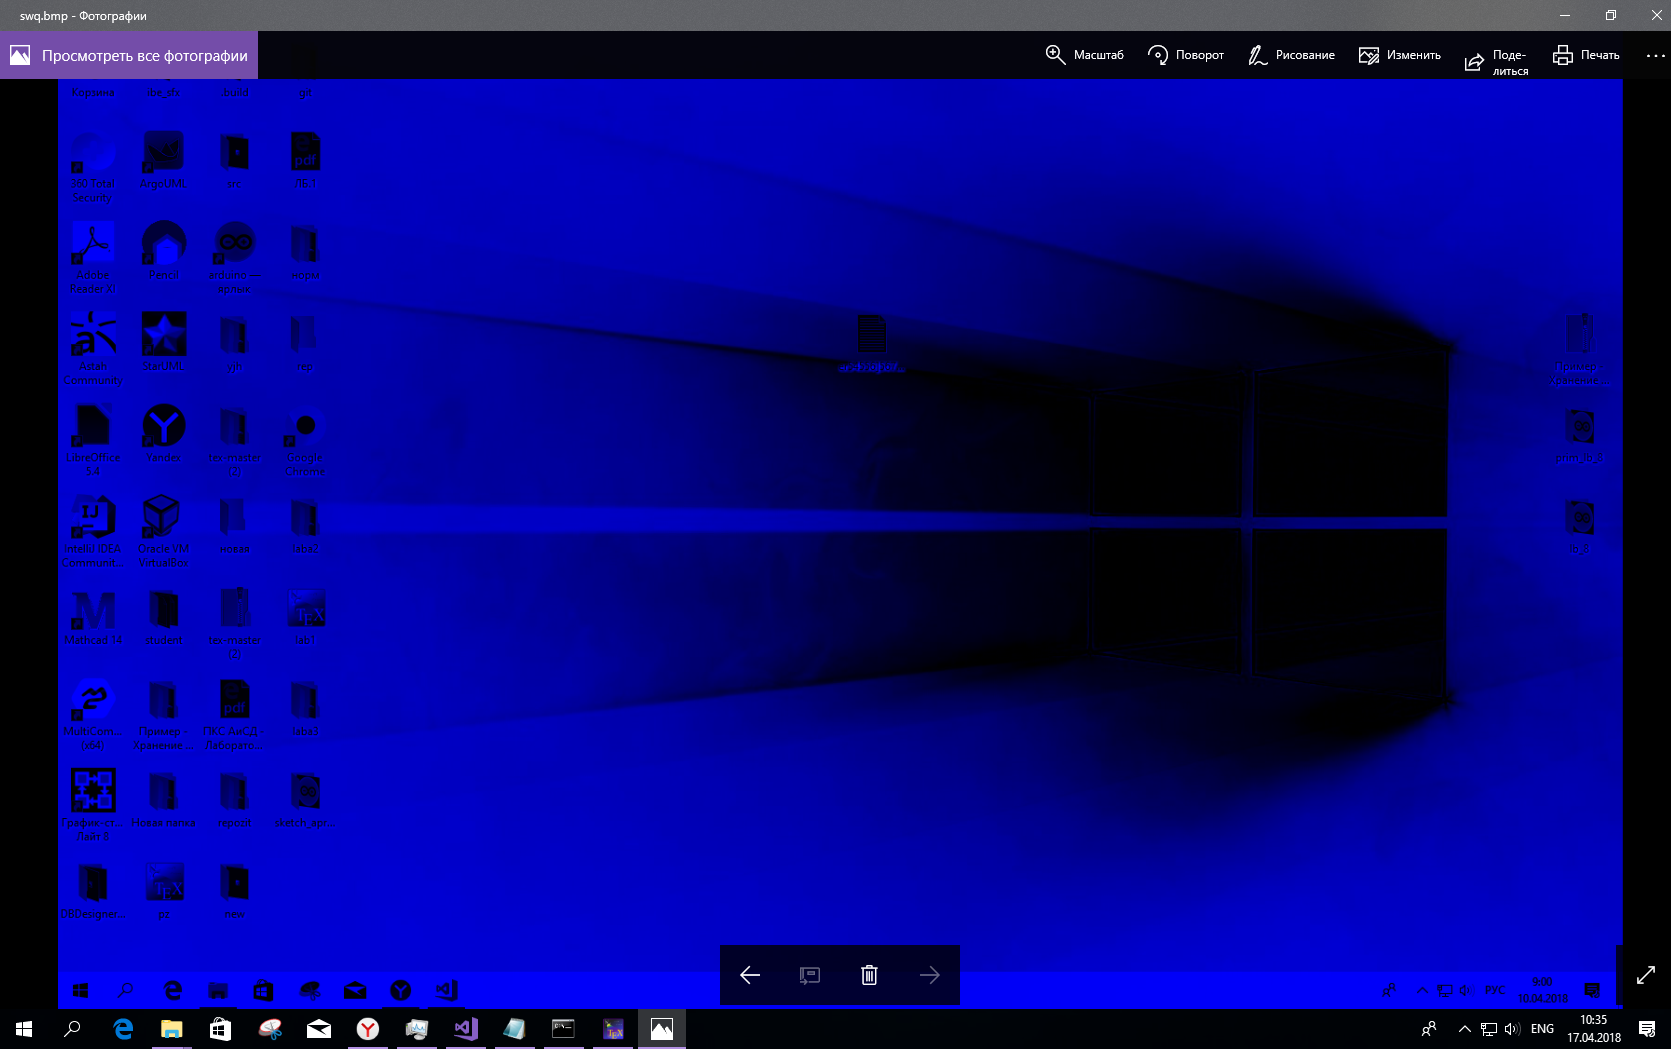
\includegraphics[scale=0.4]{ght}
\caption{Результат}
\label{fig:ght}
\end{figure}


\textbf{Вывод:} Я научился работать с пакетами для с++;



